
\chapter{Relatividad Especial}

\section{Principio de relatividad}
\begin{frame}[fragile,allowframebreaks]
El \emph{principio de relatividad} establece que:
\begin{quote}
  Las leyes de la física tienen la misma forma en todos los sistemas inerciales. 
\end{quote}
Esto generaliza lo que se conoce de la mecánica en donde si en un sistema inercial $S$ el principio de moméntum  es $\mathbf{F}=d\mathbf{P}/dt$, en un sistema inercial $S'$, será $\mathbf{F}'=d\mathbf{P}'/dt$.
\end{frame}
\section{Transformaciones de Lorentz}
\begin{frame}[fragile,allowframebreaks]
Sea el sistema de referencia $S'$ moviendose a lo largo del eje $x$ con rapidez $V$ relativa al sistema de referencia estacionario de referencia $S$ como se muestra en la figura~\ref{fig:lorentz}
\begin{figure}
  \centering
  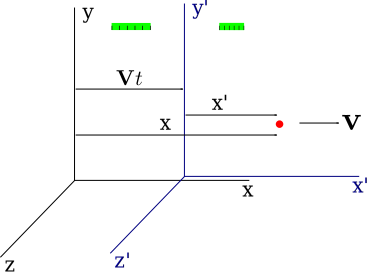
\includegraphics[scale=0.7]{lorentz}
  \caption{Transformaciones entre sistemas inerciales}
  \label{fig:lorentz}
\end{figure}

\begin{details}
Cuando se consolidaron las leyes electromagnéticas parecía como si
estas leyes dependieran del sistema inercial donde se encuentra el
observador. De hecho, una carga eléctrica por el mero hecho de estar
en movimiento, así fuese con velocidad constante, generaba campos
magnéticos. Pero, otro observador que vea la misma carga en reposo, no
vería el correspondiente campo magnético. Para que el campo magnético
y sus correspondientes leyes sean invariantes bajo diferentes
observadores inerciales se requiere bien sea proponer un éter
electromagnético ó alterar las transformaciones de Galileo. A partir
de este punto tomaremos la segunda opción que ha resultado ser la más
simple para explicar los resultados experimentales, como el
experimento de Michelson y Morley.
\end{details}

Cuando escribimos las transformaciones de Galileo
\begin{align*}
  x=Vt+x'\nonumber\\
  t=t'\,.
\end{align*}



Se ésta asumiendo que la regla de metro no cambia su longitud por estar en movimiento, pero esto no es del todo obvio. 
\begin{details}
De los fenómenos electromagnéticos que las cargas eléctricas en reposo generan campos eléctricos, mientras que las cargas eléctricas en movimiento generan además campos magnéticos. Además con el movimiento los campos eléctricos se deforman. Como la fuerzas eléctricas son importante para moldear la estructura atómica de la materia, podría en principio esperarse que la forma de la regla de metro cambia su configuración y de aquí so forma (longitud) por estar en movimiento. 
\end{details}




Entonces, admitiendo esta posibilidad, cambiaremos la Transformación de Galileo por la transformación más general:
\begin{align}
  \label{eq:gammafactor}
  x=Vt+\frac{1}{\alert{\alert{\gamma(V^2)}}} x'\,,
\end{align}
donde el factor de escala $\alert{\gamma(V^2)}$ da cuenta del posible cambio de longitud en la regla de metro en el sistema $S'$, como se ilustra en la Figura~\ref{fig:lorentz}. 
La dependencia de $\gamma$ en sólo la magnitud de la velocidad relativa dan cuenta del \emph{principio de relatividad} y de la isotropía del espacio. Además $\gamma$ debe ser adimensional.

De la ec.\eqref{eq:gammafactor}
\begin{align}
\label{eq:genltxp}
  x'=\alert{\gamma(V^2)}(x-V t)\,.
\end{align}
\begin{details}
El principio de relatividad nos dice que la misma relación se mantiene si las coordenadas primadas son cambiadas por las coordenadas sin primar, con $V$ reemplazado por $-V$, debido a que la velocidad de $S$ con respecto a $S'$ es $-V$. Además como en general las medidas de distancia en $S'$ son diferentes, no podemos asumir que el tiempo sea el mismo. Por consiguiente
\end{details}
\begin{onlybeamer}
  \begin{align*}
    x\longleftrightarrow& x'\\
    t\longleftrightarrow& t'\\
    V\longleftrightarrow& V'=-V\\
  \end{align*}
\end{onlybeamer}
\begin{align*}
    x=&\alert{\gamma(V^2)}(x'+V t')\nonumber\\
    =&\alert{\gamma}\left[\alert{\gamma}(x-V t)+V t'\right]
\end{align*}
Despejando en términos de $t'$ %detalles
\begin{align}
  \label{eq:genlttp}
  t'=\alert{\gamma}\left[t-\frac{1-\alert{\gamma^{-2}}}{V}x\right]
\end{align}
Derivando \eqref{eq:genltxp}, \eqref{eq:genlttp} obtenemos la \emph{Ley de adición de velocidades} %detalles
\begin{align*}
  v_{x'}=\frac{v_x-V}{1-\frac{1-\alert{\gamma^{-2}}}{V}v_x}
\end{align*}
la cual debe satisfacer el principio de relatividad, por lo tanto, al cambiar al sistema no primado debe mantener su forma ($V\to -V$)
\begin{align}
  \label{eq:adicionvel}
  v_{x}=\frac{v_{x'}+V}{1+\frac{1-\alert{\gamma^{-2}}}{V}v_{x'}}\,.
\end{align}
Definimos
\begin{align*}
  F(v_{x'},V)\equiv\frac{v_{x'}+V}{1+\frac{1-\alert{\gamma^{-2}}}{V}v_{x'}}
\end{align*}
\end{frame}
\subsection{Propiedades de $F(v_{x'},V)$}
\begin{frame}[fragile,allowframebreaks]
\begin{itemize}
\item \textbf{Paridad:}
  \begin{align}
    \label{eq:paridad}
    F(-v_{x'},-V)=-F(v_{x'},V)
  \end{align}
%demostración
\item \textbf{Asociatividad}
  \begin{align}
    \label{eq:asociatividad}
    v_{CA}=F(v_{CB},v_{BA})=-v_{AC}=-F(v_{AB},v_{BC})
  \end{align}
%demostración
\item \textbf{Intercambio:}
  \begin{align}
    \label{eq:intercambio}
    F(v_{CB},v_{BA})=F(v_{BA},v_{CB})
  \end{align}
\textbf{Demostración:} Usando ecs.~\eqref{eq:paridad}\eqref{eq:asociatividad}

\end{itemize}
\end{frame}
\section{Soluciones}

\begin{frame}[fragile,allowframebreaks]
Entonces
\begin{align*}
  F(v_{x'},V)=F(V,v_{x'})\,.
\end{align*}
Obtenemos %detalles
\begin{align*}
  \Gamma=\frac{1-\alert{\gamma^{-2}(V^2)}}{\alert{V^2}}=\text{constante} \alert{\text{\qquad Independiete de $V^2$}!!!}
\end{align*}
Por las dimensiones de $\Gamma$ podemos definir
\begin{align*}
  \Gamma=\frac{1}{c^2}\,.
\end{align*}

\subsection{$\Gamma >0$}
%detalles
\begin{align*}
  \gamma=&\frac{1}{\sqrt{1-\Gamma V^2}}\nonumber\\
  \alert{\gamma=}&\alert{\frac{1}{\sqrt{1-V^2/c^2}}}\,,
\end{align*}
de modo que si $\Gamma>0$ entonces $\gamma>1$. las \emph{Transformaciones de Lorentz} quedan
\begin{align}
  \label{eq:lorentz}
  x'=&\alert{\gamma}(x-V t)\nonumber\\
  t'=&\alert{\gamma}\left(t-\frac{V}{c^2}x\right)
\end{align}
Mientras que las transformaciones inversas son
\begin{align}
  \label{eq:lorentzinv}
  x=&\alert{\gamma}(x'+V t')\nonumber\\
  t=&\alert{\gamma}\left(t'+\frac{V}{c^2}x'\right)\,.
\end{align}


Las Transformaciones de Lorentz  a lo largo del eje $x$ se pueden escribir en forma matricial como
\begin{equation}
\label{eq:147qft}
  \begin{pmatrix}
    ct\\
    x\\
    y\\
    z
  \end{pmatrix}\to
  \begin{pmatrix}
    ct'\\
    x'\\
    y'\\
    z'
  \end{pmatrix}=
  \begin{pmatrix}
    \frac{ct-Vx}{\sqrt{1-V^2/c^2}}\\
    \frac{x-Vct}{\sqrt{1-V^2/c^2}}\\
    y\\
    z
  \end{pmatrix}=
  \begin{pmatrix}
    \cosh\xi&\sinh\xi&0&0\\
    \sinh\xi&\cosh\xi&0&0\\
    0     &  0  &1&0\\
    0     &  0  &0&1
  \end{pmatrix}
  \begin{pmatrix}
    ct\\
    x\\
    y\\
    z
  \end{pmatrix}
\end{equation}
donde
\begin{equation}
  \cosh\xi=\alert{\gamma}\qquad\sinh\xi=-\alert{\gamma} V/c\,,
\end{equation}
\begin{align*}
\cosh^2\xi-\sin^2\xi=&1\nonumber\\
\alert{\gamma}^2(1-V^2/c^2)=&1\nonumber\\
 \alert{\gamma}=&\frac{1}{\sqrt{1-V^2/c^2}}.
\end{align*}
y, por ejemplo:
\begin{align}
ct'=  ct\cosh{\xi}+x\sinh\xi=\alert{\gamma}(ct-V x/c)=&c\frac{t-V x/c^2}{\sqrt{1-V^2/c^2}}\nonumber\\
t'=  t\cosh{\xi}+x\sinh\xi=\alert{\gamma}(ct-V x/c)/c=&\frac{t-V x/c^2}{\sqrt{1-V^2/c^2}}\nonumber\\
x'=  ct\sinh{\xi}+x\cosh\xi=\alert{\gamma}(-Vt+ x)=&\frac{x-Vt}{\sqrt{1-V^2/c^2}}\,.
\end{align}

\end{frame}
\subsection{Ley de adición de velocidades}
\begin{frame}[fragile,allowframebreaks]
Teniendo en cuenta que
\begin{align*}
  \alert{\gamma}^{-2}=1-\frac{V^2}{c^2}\,,
\end{align*}
la ley de adición de velocidades \eqref{eq:adicionvel} queda
\begin{align*}
  F(v_{x'},V)=v_{x}=&\frac{v_{x'}+V}{1+\frac{1-\alert{\gamma}^{-2}}{V}v_{x'}}\nonumber\\
  =&\frac{v_{x'}+V}{1+\frac{1-1+V^2/c^2}{V}v_{x'}}\nonumber\\
  =&\frac{v_{x'}+V}{1+{Vv_{x'}}/{c^2}}\,,
\end{align*}
La relación inversa es por consiguiente
\begin{align}
  \label{eq:addvel}
v_{x'}=\frac{v_x-V}{1-V v_x/c^2}\,.
\end{align}
En ausencia de una velocidad límite, es decir cuando $c\to \infty$, o equivalentemente, cuando $V\ll c$, obtenemos el resultado Galileano
\begin{align}
  \label{eq:galsumavel}
  v_{x'}=v_x-V\,.
\end{align}


\begin{itemize}
\item[\textbf{Ejemplo:}] En un futuro muy lejano, una nave espacial llamada Enterprise sale hacia una dirección en ele espacio exterior con una rapidez de $0.9c$, al mismo tiempo una nave llamada Fleagle sale en dirección opuesta con rapidez de $0.9c$. Calcular la velocidad relativa entre ellas.
  \begin{figure}
    \centering
    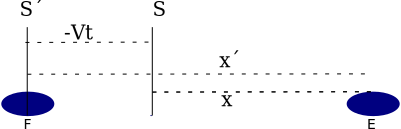
\includegraphics{enterprise}
    \caption{Sistemas de referencias en reposo $S$ y en movimiento $S'$. La nave Feagle está en el origen de $S'$.}
    \label{fig:enterprise}    
  \end{figure}
\item[\textbf{Solución}].  Sea $\mathbf{v}=v_x\hat{\mathbf{i}}=0.9c\,\hat{\mathbf{i}}$ la velocidad de la Enterprise relativa a un sistema en reposo $S$, y $\mathbf{V}=-0.9c\,\hat{\mathbf{i}}$, la velocidad de Fleagle relativa al sistema $S$ como se muestra en la figura~\ref{fig:enterprise}. La velocidad de la Entreprise relativa a la Fleage es $v_{x'}$, es decir, la velocidad con la cual un observador en la Fleagle ve alejarse a la Enterprise. Si no existiese una velocidad límite, la velocidad relativa entre las naves sería (ver \eqref{eq:galsumavel}) de $v_{x'}=1.8\,c$. Sin embargo, usando la Ley de adición de velocidades \eqref{eq:addvel}
  \begin{align*}
    v_{x'}=&\frac{0.9c-(-0.9c)}{1-[(-0.9c)(0.9c)/c^2]}\nonumber\\
    =&\frac{1.8c}{1.81}\nonumber\\
    =&0.99c\,.
  \end{align*}

La velocidad relativa es menor que $c$. La transformaciones relativística de velocidades asegura que no podemos exceder la velocidad de la luz cambiando los sistemas de referencia. 
\end{itemize}

Sea $\mathbf{v}=v_{x}=c\,\hat{\mathbf{i}}$ la velocidad límite de un cuerpo relativa a un sistema en reposo $S$ como el que se ilustró en el ejemplo anterior en la figura~\ref{fig:enterprise}. Consideremos un observador en el origen de un sistema $S'$ que se muve con \emph{cualquier} rapidez $V$ que incluso podría ser $c$, y en cualquier sentido ($\pm V$). La velocidad con la cual el observador en $S'$ ve moverse el cuerpo es, de acuerdo a  la Ley de adición de velocidades \eqref{eq:addvel}:
\begin{align*}
  v_{x'}=&\frac{c-(\pm V)}{1-(\pm V)c/c^2}\nonumber\\
  =&\frac{c\mp V}{1\mp V/c}\nonumber\\
  =&\frac{c\mp V}{(c\mp V)/c}\nonumber\\
  v_{x'}=&c\,.
\end{align*}
Por consiguiente, una consecuencia de la Ley de adición de velocidades es que:
\begin{quote}
  La velocidad límite $c$, es la misma para todos los observadores inerciales.
\end{quote}

\end{frame}
\subsection{Simultaneidad y orden de eventos}

\begin{frame}[fragile,allowframebreaks]
Un evento esta caracterizado por un conjunto de valores para las coordenadas $x,y,z,t$.  Con respecto a un sistema de coordenadas dado, dos eventos son \emph{simultáneos} si sus coordenadas temporales tienen el mismo valor
\end{frame}

\subsection{Contracción de Lorentz}
\begin{frame}[fragile,allowframebreaks]
Como hemos visto, la existencia de una velocidad límite en la naturaleza, la cual hemos identificaremos de ahora en adelante con la velocidad de la luz, afecta la forma de los cuerpos. Para ver las implicaciones de tener $\alert{\gamma}>0$ en un cuerpo en movimiento primero definimos el sistema $S:(x,y,z,t)$ como sistema de laboratorio, y consideremos una varilla en reposo en el sistema $S':(x',y',z',t')$ que se mueve con velocidad rapidez $v$ respecto a $S$. 

Definimos la longitud de la varilla como la distancia entre sus extremos en el mismo instante de tiempo. Los puntos finales deben ser determinados simultáneamente en el sistema de laboratorio; y debemos encontrar la relación entre $x'$ y $x$ para ese valor de $t$. Tenemos
\begin{align*}
  x'=\alert{\gamma}(x-vt)\,.
\end{align*}
Para cada extremo de la varilla, al tiempo $t$ de los eventos simultáneos en los que se determina la posición de los extremos de la varilla desde el sistema de laboratorio, es
\begin{align*}
  x'_A=&\alert{\gamma}(x_A-vt)\nonumber\\
  x'_B=&\alert{\gamma}(x_B-vt)\,,
\end{align*}
Restando ambas ecuaciones, obtenemos
\begin{align*}
  l'=l_0\equiv=x'_B-x'_A=\alert{\gamma}(x_B-x_A)=\alert{\gamma} l\,,
\end{align*}
donde $l_0$ es la longitud en reposo o \emph{propia} de la varilla, y $l$ es la longitud medida en el laboratorio para una varilla en movimiento a velocidad $v$. Entonces
\begin{align*}
  l=\frac{l_0}{\alert{\gamma}}=l_0\sqrt{1-\frac{v^2}{c^2}}\,,
\end{align*}
de modo que $l$ es más corta que $l_0$, la varilla se contrae. A medida que $v\to c$, $l\to 0$. Es importante notar que dicha longitud es relativa al observador en el sistema de laboratorio desde donde los extremos de la varilla se han medido simultáneamente. Un observador en reposo respecto a la varilla no nota ningún cambio en su longitud.
\end{frame}
\subsection{Dilatación temporal}
\begin{frame}[fragile,allowframebreaks]
Consideremos un reloj en reposo en el sistema $x',y',z'$ y considere dos eventos $A$ y $B$ ambos ocurriendo en el mismo punto $x_0'$:
\begin{align*}
  A:(x_0',t_A')\nonumber\\
  B:(x_0',t_B')\nonumber\\
\end{align*}
El intervalo $\tau=t_B'-t_A'$ es el intervalo temporal entre los eventos en el sistema $S'$ donde el reloj está en reposo. Dicho sistema se mueve con rapidez $v$ respecto al sistema de laboratorio $S$, relacionado con $S'$ por (ec.~\eqref{eq:lorentzinv})
\begin{align*}
  t=\alert{\gamma}\left(t'+\frac{V}{c^2}x'\right)
\end{align*}
de modo que
\begin{align*}
   t_A=&\alert{\gamma}\left(t_A'+\frac{V}{c^2}x_0'\right)\nonumber\\
   t_B=&\alert{\gamma}\left(t_B'+\frac{V}{c^2}x_0'\right)\,,
\end{align*}
restando, encontramos
\begin{align*}
  T=t_B-t_A=&\alert{\gamma}(t_B'-t_A')\nonumber\\
  =&\alert{\gamma}\tau\nonumber\\
  =&\frac{\tau}{\sqrt{1-v^2/c^2}}\,.
\end{align*}

El intervalo temporal en el sistema de laboratorio es más grande que en el sistema en reposo, de modo que un reloj en movimiento se mueve más lento. Este efecto es conocido como la dilatación temporal y tiene importantes consecuencias prácticas.

\begin{itemize}
\item[\textbf{Ejemplo:}] \textbf{Decaimiento del muón} El muón decae a través de la interacciones débiles a un electrón, un neutrino muónico, y un antineutrino tau con un tiempo de vida media de $\tau=2.15\times 10^{-6}\second$. De modo que si decae en reposo recorre una distancia promedio de
  \begin{align*}
    d=c\tau\approx 3\times 10^8\times 2.15\times 10^{-6}=645\meter\,. 
  \end{align*}
Si un muón se genera en la atmósfera con un $\alert{\gamma}=10$, ¿que distancia promedio recorre antes de decaer?.
\item[\textbf{Solución:}] Cuando el muón se mueve rápidamente, el tiempo de vida $\tau'$ que se observa desde un laboratorio en la superficie de la tierra, se incrementa por la dilatación temporal. El tiempo de vida observado es
  \begin{align*}
    \tau'=&\alert{\gamma}\tau\,,
  \end{align*}
de modo que
\begin{align*}
  d'=c\tau'=\alert{\gamma} c\tau=10 c\tau\approx 6450\meter\,,
\end{align*}
la dilatación temporal permite que los muones puedan llegar a la superficie de la tierra a un tasa de 10,000 muones por metro cuadrado cada minuto ( Mark Wolverton (September 2007). "Muons for Peace: New Way to Spot Hidden Nukes Gets Ready to Debut". Scientific American 297 (3): 26–28.), a pesar de producirse en la partes altas de la atmósfera.
\end{itemize}
%otras soluciones
\end{frame}

\begin{frame}[fragile,allowframebreaks]
\section{Momento energía}
Supongamos que para una colisión
\begin{align*}
  p=m(v)\mathbf{v}
\end{align*}
donde $m(v)$ debe determinarse. Del estudio de colisiones
\begin{align*}
  m(v)=\alert{\gamma} m_0\,,
\end{align*}
donde $m_0$ es la masa en reposo de la partícula. (Ver Jackson por ejemplo)

De este modo, la expresión correcta para el moméntum es
\begin{align}
  \label{eq:gmv}
  p=\alert{\gamma} m_0 \mathbf{v}\,,  
\end{align}


Para obtener la energía consideremos el trabajo
\begin{align*}
  W_{ba}=&\int\frac{d\mathbf{p}}{dt}\cdot d\mathbf{r}\nonumber\\
  =&\int\left[d(\mathbf{p}\cdot\frac{d\mathbf{r}}{dt})-\mathbf{p}\cdot d\left(\frac{\mathbf{dr}}{dt}  \right)\right]\nonumber\\
=&\mathbf{v}\cdot \mathbf{p}|_a^b-\int_a^b\mathbf{p}\cdot d\mathbf{v}\nonumber\\
=&\mathbf{v}\cdot (\alert{\gamma} m_0\mathbf{v})|_a^b-\int_a^b\alert{\gamma} m_0\mathbf{v}\cdot d\mathbf{v}\nonumber\\
=&\left.\frac{m_0 v^2}{\sqrt{1-{v^2}/{c^2}}}\right|_a^b-\int_a^b\frac{m_0v dv}{\sqrt{1-v^2/c^2}}\nonumber\\
=&\left.\frac{m_0 v^2}{\sqrt{1-{v^2}/{c^2}}}\right|_a^b+\left.m_0 c^2\sqrt{1-\frac{v^2}{c^2}}\right|_a^b
\end{align*}
donde hemos usado que
\begin{align*}
  \frac{d}{dv}
  \left(
    1-\frac{v^2}{c^2}
  \right)=&\frac{1}{2}\frac{2v}{c^2}
  \left(1-\frac{v^2}{c^2}\right)^{-1/2}\nonumber\\
  =&\frac{v}{c^2}\frac{1}{\sqrt{1-{v^2}/{c^2}}}
\end{align*}

Sea $a$, tal que $v_a=0$ y $v_b=v$, entonces
\begin{align*}
  W_{ba}=&\frac{m_0 v^2}{\sqrt{1-v^2/c^2}}+m_0 c^2\sqrt{1-\frac{v^2}{c^2}}-m_0 c^2\nonumber\\
=&\frac{\cancel{m_0 v^2}+m_0c^2(1-\cancel{v^2/c^2})}{\sqrt{1-v^2/c^2}}-m_0 c^2\nonumber\\
=&\frac{m_0c^2}{\sqrt{1-v^2/c^2}}-m_0 c^2\nonumber\\
  =&mc^2-m_0 c^2
\end{align*}

Cuando $v\ll c$
\begin{align*}
 W_{ba} =&\frac{m_0c^2}{\sqrt{1-v^2/c^2}}-m_0 c^2\nonumber\\
\approx&{m_0c^2}\left(1-\frac{(-1)}{2}\frac{v^2}{c^2}\right)-m_0 c^2\nonumber\\
\approx&{m_0c^2}+\frac{1}{2}m_0{v^2}-m_0 c^2\nonumber\\
\approx&\frac{1}{2}m_0{v^2}\nonumber\\
\approx&K\nonumber\\
\approx&\text{energía cinética}\,.
\end{align*}
Ya que el término $m_0c^2$ lo podemos interpretar como la energía en reposo de la partícula, el trabajo completo $W_{ba}$, lo  podemos interptretar como
\begin{align*}
  W_{ba}=\text{Energía cinética relativista}=\text{Energía total}-\text{Energía en reposo}
\end{align*}
donde definimos la \emph{energía total} de una partícula, $E$, como
\begin{align}
  \label{eq:gme}  
  E=&\frac{m_0c^2}{\sqrt{1-v^2/c^2}}\nonumber\\
  =&\alert{\gamma} m_0c^2\,,
\end{align}
es decir, $\alert{\gamma}$ veces la energía en reposo.

Note que la energía total depende de $v^2$
\begin{align}
  E(v^2)=\frac{m_0c^2}{\sqrt{1-v^2/c^2}}\nonumber\\
  =E(0)+K
\end{align}
donde $E(0)$ es la energía en reposo.

Combinando la ec.~\eqref{eq:gmv} con \eqref{eq:gme}, tenemos
\begin{align}
  \frac{E^2}{c^2}-\mathbf{p}^2=&\alert{\gamma}^2 m_0^2 c^2-\alert{\gamma}^2 m_0^2 v^2\nonumber\\
  =&m_0^2 \alert{\gamma}^2(  c^2- v^2)\nonumber\\
  =&m_0^2 c^2 \alert{\gamma}^2( 1- v^2/c^2)\nonumber\\
  =&m_0^2 c^2\,,
\end{align}
De modo que
\begin{align}
  E^2-c^2\mathbf{p}^2=m_0^2 c^4
\end{align}
y si tomamos un sistema de unidades done $c=1$
\begin{align}
  E^2-\mathbf{p}^2=m_0^2\,,\qquad c=1\,.
\end{align}
En este sistema de unidades
\begin{align}
  [E]=[|\mathbf{p}|]=[m_0]\,.
\end{align}
Además una longitud $L$ y un tiempo $T$ tienen unidades
\begin{align}
  [L]=[T]=[E]^{-1}\,.
\end{align}

Por ejemplo la masa del protón, y otras partículas subatómicas como el quark top, el bosón gauge $Z$, o el bosón de Higgs, son respectivamente
\begin{align*}
  m_p\approx &1\ \text{GeV}\\
  m_t\approx& 175\ \text{GeV}\\
  m_Z\approx& 91\ \text{GeV}\\
  m_H\approx& 125\ \text{GeV}\,,
\end{align*}
donde
\begin{align*}
  1\ \text{eV}=\SI{1.60217646\times 10^{-19}}{\joule}
\end{align*}

% \begin{align*}
%   mc^2=&W_{ba}+m_0c^2\nonumber\\
% =&\text{Trabajo hecho sobre la partícula}+m_0c^2
% \end{align*}
% donde $E=mc^2=\frac{m_0c^2}{\sqrt{1-v^2/c^2}}$, es la energía total de la partícula. Cuando $v\ll c$,
% \begin{align*}
%   K\approx \frac{1}{2}m_0 v^2\,.
% \end{align*}
\end{frame}
\section{Notación relativista}
\label{sec:srn}
Las transformaciones de Lorentz se definen como la transformaciones que dejan invariante al producto escalar en el espacio de Minkowski definido como
\begin{equation}
  \label{eq:146qft}
  a^2=g_{\mu\nu}a^\mu a^\nu\equiv a_\nu a^\nu={a^0}^2-a^i a^i={a^0}^2-\mathbf{a}\cdot\mathbf{a}
\end{equation}
donde $\mu,\nu=0,1,2,3$, $i=1,2,3$ y se asume suma sobre índices repetidos. Además
\begin{equation}
\label{eq:149qft}
  a_\nu\equiv g_{\mu\nu}a^\mu
\end{equation}
 Finalmente la métrica usada se define como
\begin{equation}
  \label{eq:gmunu}
  \left\{ g_{\mu\nu} \right\}=
  \begin{pmatrix}
    1&0&0&0\\
    0&-1&0&0\\
    0&0&-1&0\\
    0&0&0&-1
  \end{pmatrix}
\end{equation}
donde $\left\{ g_{\mu\nu} \right\}$ denota la forma matricial del tensor $g_{\mu\nu}$.  

El producto de dos cuadrivectores se define en forma similar como
\begin{equation}
\label{eq:157qft}
  a_\nu b^\nu=g_{\mu\nu}a^\mu b^\nu=a^0b^0-\mathbf{a}\cdot\mathbf{b}
\end{equation}
El inverso de la métrica es
\begin{equation}
  \left\{ g^{\mu\nu} \right\}\equiv\left\{ g_{\mu\nu} \right\}^{-1}=\left\{ g_{\mu\nu} \right\}
\end{equation}
tal que
\begin{equation}
  g^{\mu\alpha}g_{\alpha\nu}=\delta^\mu_\nu\qquad\text{and}\qquad a^\mu=g^{\mu\nu}a_\nu
\end{equation}

Bajo una transformación de Lorentz.
\begin{align}
  a^\mu\to {a'}^\mu=&{\Lambda^\mu}_{\nu}a^\nu\\
  a_\mu\to {a'}_\mu=&{\Lambda_\mu}^{\nu}a_\nu\nonumber
\end{align}
La invarianza del producto escalar en ec.~\eqref{eq:157qft}
\begin{align}
  {a'}^\mu{b'}_\mu=&a^\mu b_\mu\nonumber\\
g_{\alpha\beta}{a'}^\alpha{b'}^\beta=g_{\mu\nu}a^\mu b^\nu\nonumber\\
g_{\alpha\beta}{\Lambda^\alpha}_\mu{a}^\mu{\Lambda^\beta}_\nu{b}^\nu=g_{\mu\nu}a^\mu b^\nu\nonumber\\
{\Lambda^\alpha}_\mu g_{\alpha\beta}{\Lambda^\beta}_\nu{a}^\mu{b}^\nu=g_{\mu\nu}a^\mu b^\nu\,,
\end{align}
da lugar a
\begin{equation}
  \label{eq:lrinv}
  g_{\mu\nu}={\Lambda^\alpha}_{\mu}g_{\alpha\beta}{\Lambda^\beta}_{\nu}\qquad\text{or}\qquad 
\left\{g_{\mu\nu}\right\}=\left\{{\Lambda_{\mu}}^{\alpha}\right\}^{\text{T}}\left\{g_{\alpha\beta}\right\}\left\{{\Lambda^\beta}_{\nu}\right\}.
\end{equation}
En notación matricial
\begin{align}
 g=\Lambda^T g \Lambda\,. 
\end{align}
From eq.~\eqref{eq:lrinv} we also have
\begin{align}
  g^{\rho\mu}g_{\mu\nu}=&g^{\rho\mu}{\Lambda^\alpha}_{\mu}g_{\alpha\beta}{\Lambda^\beta}_{\nu}\nonumber\\
  \delta^\rho_\nu=&{\Lambda_\beta}^\rho{\Lambda^\beta}_{\nu}\,,
\end{align}
or
\begin{align}
  {\Lambda_\alpha}^\mu{\Lambda^\alpha}_{\nu}=\delta^\mu_\nu\,.
\end{align}
Since
\begin{align}
  {\left(\Lambda^{-1}\right)^\mu}_\alpha{\Lambda^\alpha}_{\nu}=\delta^\mu_\nu\,
\end{align}
the inverse of $\Lambda$ is
\begin{align}
  {\left(\Lambda^{-1}\right)^\mu}_\alpha={\Lambda_\alpha}^\mu\,,
\end{align}
or
\begin{align}
\label{eq:lambdainv}
  {\left(\Lambda^{-1}\right)^\mu}_\nu={\Lambda_\nu}^\mu\,,
\end{align}
\begin{itemize}
\item \textbf{Example:} Lorentz invariance
  \begin{align}
    a_\mu b^\mu\to a'_\mu{b'}^\mu=&{\Lambda_\mu}^\nu a_\nu{\Lambda^\mu}_\rho b^p \nonumber\\
    =&{\Lambda_\mu}^\nu a_\nu{\Lambda^\mu}_\rho b^p \nonumber\\
    =&{\left(\Lambda^{-1}\right)^\nu}_\mu{\Lambda^\mu}_\rho a_\nu b^p \nonumber\\
    =&\delta^\nu_\rho a_\nu b^p \nonumber\\
    =&a_\nu b^\nu \nonumber\,.
  \end{align}

\end{itemize}

Como un ejemplo de Transformación de Lorentz considere un desplazamiento a lo largo del eje $x$
\begin{equation}
\label{eq:147qft}
  \left\{x^\mu\right\}=\begin{pmatrix}
    t\\
    x\\
    y\\
    z
  \end{pmatrix}\to
  \begin{pmatrix}
    t'\\
    x'\\
    y'\\
    z'
  \end{pmatrix}=
  \begin{pmatrix}
    \frac{t+vx}{\sqrt{1-v^2}}\\
    \frac{x+vt}{\sqrt{1-v^2}}\\
    y\\
    z
  \end{pmatrix}=
  \begin{pmatrix}
    \cosh\xi&\sinh\xi&0&0\\
    \sinh\xi&\cosh\xi&0&0\\
    0     &  0  &1&0\\
    0     &  0  &0&1
  \end{pmatrix}
  \begin{pmatrix}
    t\\
    x\\
    y\\
    z
  \end{pmatrix}=\left\{{\Lambda^\mu}_{\nu}\right\}\left\{x^\nu\right\},
\end{equation}
donde
\begin{equation}
  \cosh\xi=\alert{\gamma}\qquad\sinh\xi=v\alert{\gamma},\qquad\text{and}\qquad \alert{\gamma}=\frac{1}{\sqrt{1-v^2}}.
\end{equation}
y, por ejemplo:
\begin{align}
  t\cosh{\xi}+x\sinh\xi=\alert{\gamma}(t+v x)=\frac{t+v x}{\sqrt{1-v^2}}\,.
\end{align}
El ${\Lambda^\mu}_{\nu}$ definido en la ec.~\eqref{eq:147qft} satisface la condición en ec.~\eqref{eq:148qft}, 
\begin{align}
  \Lambda^T g \Lambda=&\begin{pmatrix}
    \cosh\xi&\sinh\xi&0&0\\
    \sinh\xi&\cosh\xi&0&0\\
    0     &  0  &1&0\\
    0     &  0  &0&1
  \end{pmatrix}
  \begin{pmatrix}
    1 & 0  & 0 &0\\
    0 & -1 & 0 &0\\
    0 & 0  & -1&0\\
    0 & 0  & 0 &-1\\
  \end{pmatrix}
  \begin{pmatrix}
    \cosh\xi&\sinh\xi&0&0\\
    \sinh\xi&\cosh\xi&0&0\\
    0     &  0  &1&0\\
    0     &  0  &0&1
  \end{pmatrix}\nonumber\\
  =&\begin{pmatrix}
       \cosh\xi&-\sinh\xi&0&0\\
    \sinh\xi&-\cosh\xi&0&0\\
    0     &  0  &-1&0\\
    0     &  0  &0&-1
  \end{pmatrix}
 \begin{pmatrix}
    \cosh\xi&\sinh\xi&0&0\\
    \sinh\xi&\cosh\xi&0&0\\
    0     &  0  &1&0\\
    0     &  0  &0&1
  \end{pmatrix}\nonumber\\
  =&\begin{pmatrix}
       \cosh^2\xi-\sinh^2\xi&\cosh\xi\sinh\xi-\cosh\xi\sinh\xi&0&0\\
    \cosh\xi\sinh\xi-\cosh\xi\sinh\xi&\sinh^2\xi-\cosh^2\xi&0&0\\
    0     &  0  &-1&0\\
    0     &  0  &0&-1
  \end{pmatrix}\nonumber\\
=&g
\end{align}

Denotaremos los cuadrivectores con índices arriba como
\begin{equation}
  \label{eq:upindx}
  a^\mu=(a^0,a^1,a^2,a^3)=(a^0,\mathbf{a})
\end{equation}
Entonces el correspondiente cuadrivector con índices abajo, usando la ec.~\eqref{eq:149qft}, es
\begin{equation}
  a_\mu=(a_0,a_1,a_2,a_3)=(a^0,-a^1,-a^2,-a^3)=(a^0,-\mathbf{a}).
\end{equation}
Con esta notación, el producto escalar de cuadrivectores puede expresarse como el producto escalar de los dos vectores de cuatro componente $a^\mu$ y $a_\mu$.


%\left(\right)

%%% Local Variables: 
%%% mode: latex
%%% TeX-master: "mecanica"
%%% End: 
